 \section{Durchführung}
\label{sec:Durchführung}

\begin{figure}
  \centering
  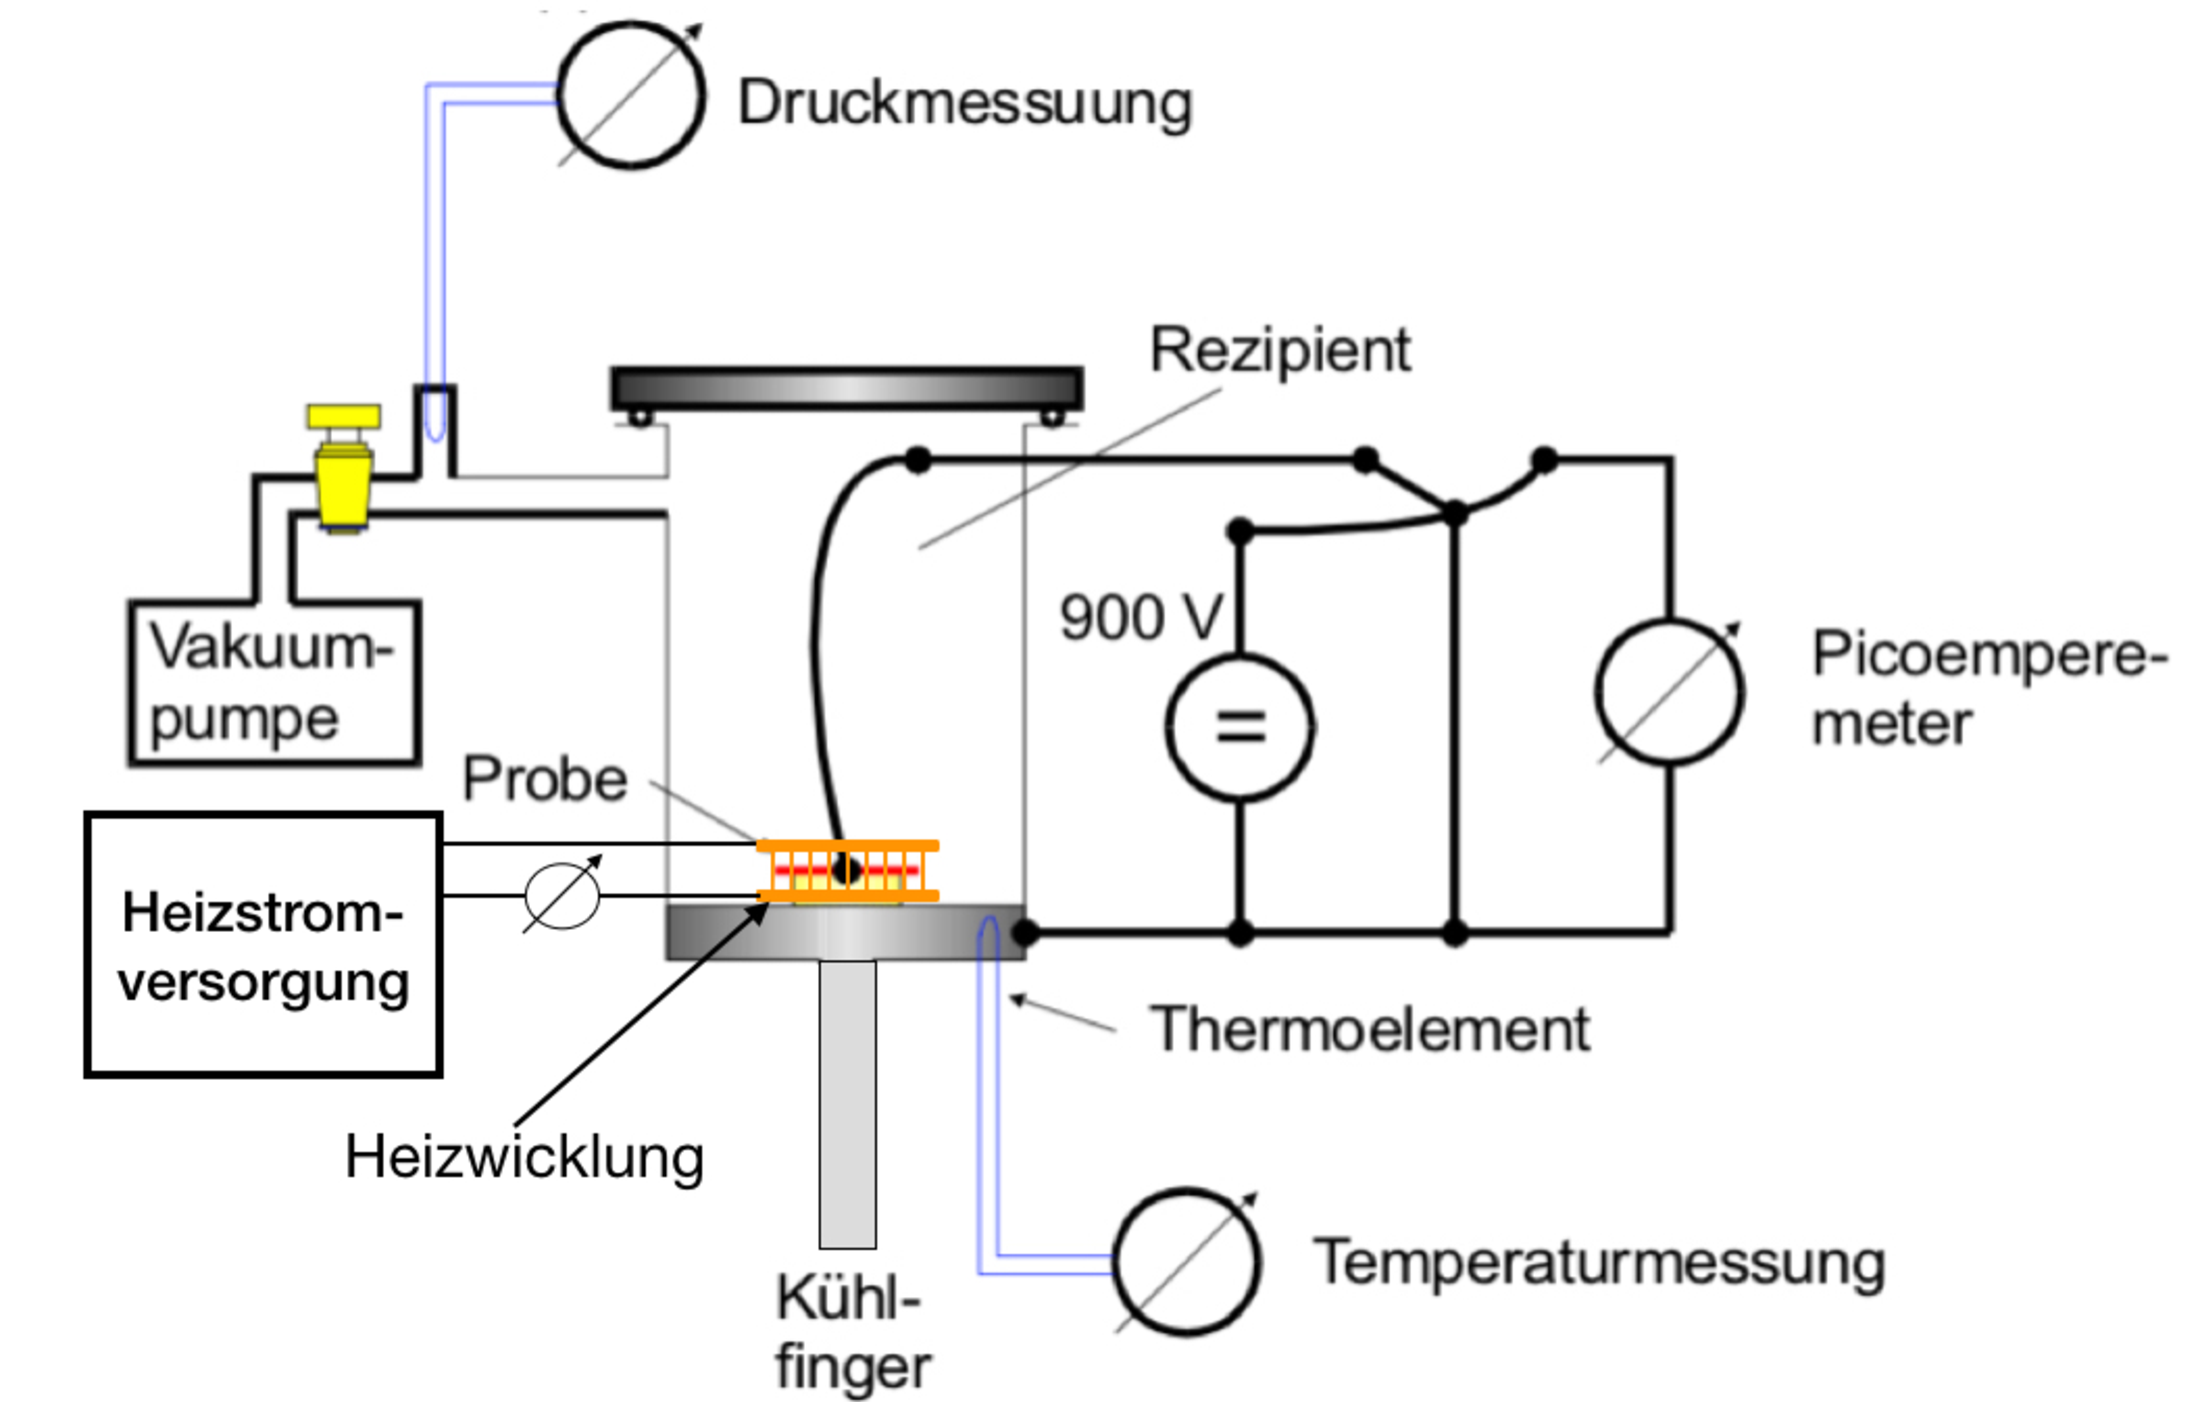
\includegraphics[height= 9cm]{BestNippelpiercings/aufbau.pdf}
  \caption{Skizze des verwendeten Aufbaus \cite{anleitung}.}
  \label{fig:aufbau}
\end{figure}
Der Aufbau des Versuchs ist in Abbildung \ref{fig:aufbau} zu sehen. Die Strom-Temperaur-Messwerte sollen nun mit zwei verschiedenen Heizraten aufgenommen werden. Dazu werden folgende Schritte durchlaufen.

\begin{itemize}
  \item Zuerst wird ein Vakuum hergestellt, damit die hygroskope Probe nicht mit Wasser bedeckt ist und so die Messung gestört ist.
  \item Dann wird mit dem Plattenkondensator eine Gleichspannung von \SI{950}{\volt} für circa \SI{900}{\second} angelegt.
  \item Als nächstes wird der Kühlfinger in flüssigen Stickstoff getaucht und die Probe so auf circa \SI{-60}{\celsius} abgekühlt.
  \item Darauf folgend wird der Kondensator für einige Minuten kurzgeschlossen.
  \item Bei der eigentlichen Messung wird dann der Heizstrom so geregelt, dass die Heizrate möglichst konstant bei \SI{2}{\celsius\per\minute} beziehungsweise \SI{1.5}{\celsius\per\minute} bleibt für die erste beziehungsweise zweite Messreihe. Gleichzeitig wird jede Minute ein Messwertpaar genommen.
\end{itemize}
